\documentclass[tikz,border=8pt]{standalone}
\usepackage{pgfplots}
\pgfplotsset{compat=1.18}
\usetikzlibrary{arrows.meta,calc,decorations.pathreplacing}
\definecolor{ink}{HTML}{17324D}
\definecolor{blue}{HTML}{1877B8}
\definecolor{orange}{HTML}{D97706}
\definecolor{green}{HTML}{16856B}
\definecolor{red}{HTML}{C24156}
\begin{document}
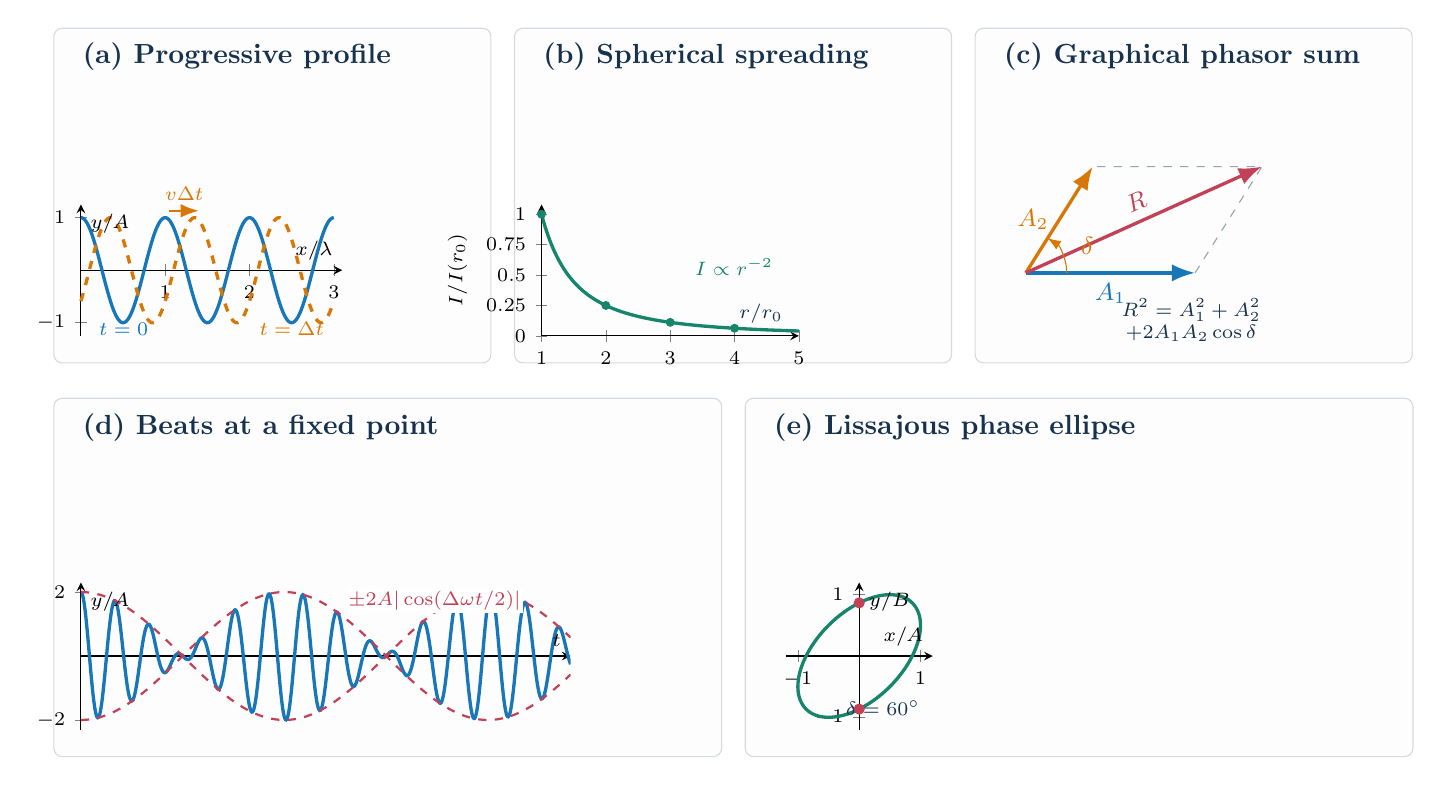
\begin{tikzpicture}[font=\small,>=Latex]
  \tikzset{panel/.style={draw=ink!18,rounded corners=3pt,fill=ink!1}}

  \node[panel,minimum width=5.55cm,minimum height=4.25cm,anchor=south west] at (0,5.0) {};
  \node[font=\bfseries,ink,anchor=west] at (0.25,8.9) {(a) Progressive profile};
  \begin{axis}[at={(0.35cm,5.35cm)},anchor=south west,width=4.9cm,height=3.25cm,
    axis lines=middle,xlabel={$x/\lambda$},ylabel={$y/A$},xmin=0,xmax=3.1,ymin=-1.25,ymax=1.25,
    xtick={0,1,2,3},ytick={-1,0,1},tick label style={font=\scriptsize},label style={font=\scriptsize},clip=false]
    \addplot[blue,very thick,domain=0:3,samples=180]{cos(deg(2*pi*x))};
    \addplot[orange,very thick,dashed,domain=0:3,samples=180]{cos(deg(2*pi*(x-0.35)))};
    \draw[->,orange,thick] (axis cs:1.05,1.13)--(axis cs:1.40,1.13) node[midway,above,font=\scriptsize] {$v\Delta t$};
    \node[blue,font=\scriptsize,anchor=west] at (axis cs:0.1,-1.12) {$t=0$};
    \node[orange,font=\scriptsize,anchor=east] at (axis cs:3.0,-1.12) {$t=\Delta t$};
  \end{axis}

  \node[panel,minimum width=5.55cm,minimum height=4.25cm,anchor=south west] at (5.85,5.0) {};
  \node[font=\bfseries,ink,anchor=west] at (6.10,8.9) {(b) Spherical spreading};
  \begin{axis}[at={(6.20cm,5.35cm)},anchor=south west,width=4.85cm,height=3.25cm,
    axis lines=left,ylabel={$I/I(r_0)$},xmin=1,xmax=5,ymin=0,ymax=1.08,
    xtick={1,2,3,4,5},ytick={0,.25,.5,.75,1},tick label style={font=\scriptsize},label style={font=\scriptsize}]
    \addplot[green,very thick,domain=1:5,samples=160]{1/x^2};
    \addplot[only marks,green,mark=*,mark size=1.4pt] coordinates {(1,1)(2,.25)(3,.1111)(4,.0625)};
    \node[green,font=\scriptsize,anchor=north east] at (axis cs:4.75,.72) {$I\propto r^{-2}$};
    \node[ink,font=\scriptsize,anchor=south east] at (axis cs:4.9,.02) {$r/r_0$};
  \end{axis}

  \node[panel,minimum width=5.55cm,minimum height=4.25cm,anchor=south west] at (11.70,5.0) {};
  \node[font=\bfseries,ink,anchor=west] at (11.95,8.9) {(c) Graphical phasor sum};
  \coordinate (O) at (12.35,6.15);
  \coordinate (P) at ($(O)+(2.15,0)$);
  \coordinate (Q) at ($(O)+(0.85,1.35)$);
  \coordinate (R) at ($(P)+(0.85,1.35)$);
  \draw[->,blue,very thick] (O)--(P) node[midway,below] {$A_1$};
  \draw[->,orange,very thick] (O)--(Q) node[midway,left] {$A_2$};
  \draw[dashed,ink!45] (P)--(R)--(Q);
  \draw[->,red,very thick] (O)--(R) node[midway,above,sloped] {$R$};
  \draw[orange,->] ($(O)+(0.52,0)$) arc[start angle=0,end angle=58,radius=.52];
  \node[orange] at ($(O)+(0.78,.34)$) {$\delta$};
  \node[align=center,font=\scriptsize,ink] at (14.45,5.55)
    {$R^2=A_1^2+A_2^2$\\$+2A_1A_2\cos\delta$};

  \node[panel,minimum width=8.48cm,minimum height=4.55cm,anchor=south west] at (0,0) {};
  \node[font=\bfseries,ink,anchor=west] at (0.25,4.18) {(d) Beats at a fixed point};
  \begin{axis}[at={(0.35cm,0.35cm)},anchor=south west,width=7.8cm,height=3.45cm,
    axis lines=middle,xlabel={$t$},ylabel={$y/A$},xmin=0,xmax=18,ymin=-2.3,ymax=2.3,
    xtick=\empty,ytick={-2,0,2},tick label style={font=\scriptsize},label style={font=\scriptsize}]
    \addplot[blue,very thick,domain=0:18,samples=700]{2*cos(deg(.42*x))*cos(deg(5*x))};
    \addplot[red,thick,dashed,domain=0:18,samples=180]{2*abs(cos(deg(.42*x)))};
    \addplot[red,thick,dashed,domain=0:18,samples=180]{-2*abs(cos(deg(.42*x)))};
    \node[red,font=\scriptsize,anchor=south,fill=white,inner sep=1pt] at (axis cs:13.0,1.32) {$\pm2A|\cos(\Delta\omega t/2)|$};
  \end{axis}

  \node[panel,minimum width=8.48cm,minimum height=4.55cm,anchor=south west] at (8.78,0) {};
  \node[font=\bfseries,ink,anchor=west] at (9.03,4.18) {(e) Lissajous phase ellipse};
  \begin{axis}[at={(9.30cm,0.35cm)},anchor=south west,width=7.1cm,height=3.45cm,
    axis equal image,axis lines=middle,xlabel={$x/A$},ylabel={$y/B$},xmin=-1.2,xmax=1.2,ymin=-1.2,ymax=1.2,
    xtick={-1,0,1},ytick={-1,0,1},tick label style={font=\scriptsize},label style={font=\scriptsize}]
    \addplot[green,very thick,domain=0:360,samples=241] ({sin(x)},{sin(x+60)});
    \addplot[only marks,red,mark=*,mark size=1.8pt] coordinates {(0,.866)(0,-.866)};
    \node[ink,font=\scriptsize,anchor=south east] at (axis cs:1.15,-1.13) {$\delta=60^\circ$};
  \end{axis}
\end{tikzpicture}
\end{document}
